\documentclass{standalone}
\usepackage{tikz}
\usepackage{ifthen}

\begin{document}
	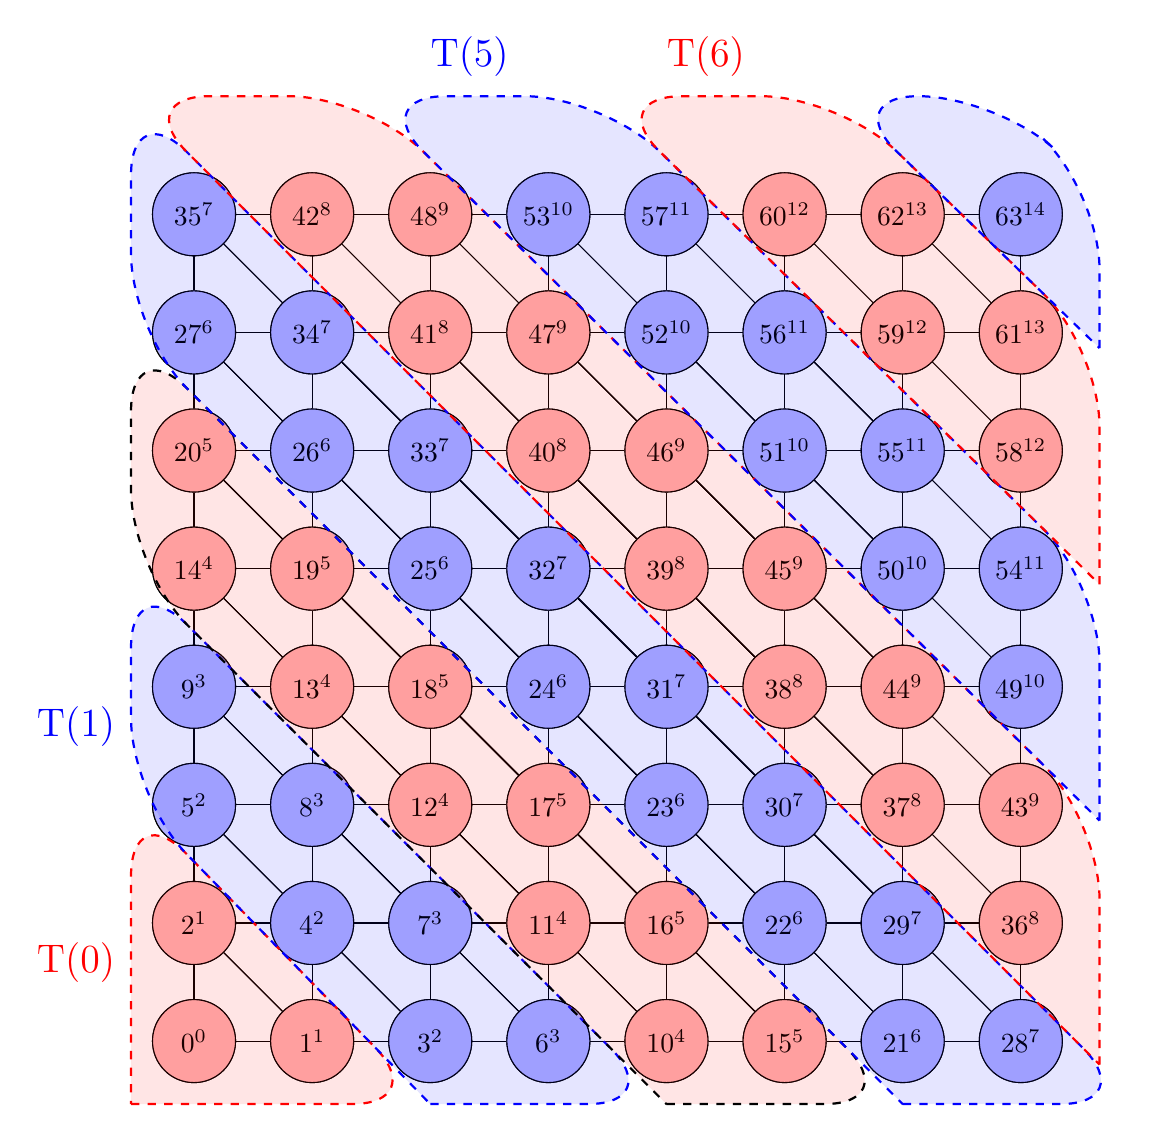
\begin{tikzpicture}[redstyle/.style={circle,draw,fill=red!30!white,minimum size=30}, bluestyle/.style={circle,draw,fill=blue!30!white,minimum size=30}]
	\foreach \x in {0,...,7}
	\foreach \y in {0,...,7} 
	{\pgfmathtruncatemacro{\labell}{(\y + \x)*(\y+\x+1)*0.5+\y  }
	\pgfmathtruncatemacro{\labelu}{63 - ((14 - \y - \x)*(14 - \y-\x + 1)*0.5+ 7-\y)  }
	\pgfmathtruncatemacro{\level}{\y + \x  }
	\pgfmathtruncatemacro{\levelhalf}{\level/2 }
	\pgfmathtruncatemacro{\yinv}{7 - \y }
	
	\pgfmathparse{Mod(\levelhalf,2)==0?1:0}
	\ifnum\pgfmathresult>0
		\node [redstyle]  (\x\y) at (1.5*\x,1.5*\y) { \ifthenelse{\x > \yinv} {\labelu$^{\large{\level}}$} {\labell$^{\large{\level}}$}} ;
	\else
		\node [bluestyle]  (\x\y) at (1.5*\x,1.5*\y) { \ifthenelse{\x > \yinv} {\labelu$^{\large{\level}}$} {\labell$^{\large{\level}}$}} ;
	\fi
	;}
	
	\foreach \x in {0,...,7}
	\foreach \y [count=\yi] in {0,...,6}  
	{
	\draw (\x\y)--(\x\yi) (\y\x)--(\yi\x) ;
	\draw (\x\y)-- (\y\x);
	}
	
	\foreach \x in {0,...,7}
	\foreach \y in {0,...,7} 
	{\pgfmathtruncatemacro{\labell}{(\y + \x)*(\y+\x+1)*0.5+\y  }
	\pgfmathtruncatemacro{\labelu}{63 - ((14 - \y - \x)*(14 - \y-\x + 1)*0.5+ 7-\y)  }
	\pgfmathtruncatemacro{\level}{\y + \x  }
	\pgfmathtruncatemacro{\levelhalf}{\level/2 }
	\pgfmathtruncatemacro{\yinv}{7 - \y }
	
	\pgfmathparse{Mod(\levelhalf,2)==0?1:0}
	\ifnum\pgfmathresult>0
	\node [redstyle]  (\x\y) at (1.5*\x,1.5*\y) { \ifthenelse{\x > \yinv} {\labelu$^{\large{\level}}$} {\labell$^{\large{\level}}$}} ;
	\else
	\node [bluestyle]  (\x\y) at (1.5*\x,1.5*\y) { \ifthenelse{\x > \yinv} {\labelu$^{\large{\level}}$} {\labell$^{\large{\level}}$}} ;
	\fi
	;}
	
	\draw [fill=red, fill opacity=0.1, red,dashed,rounded corners=10mm, thick] (-0.8,-0.8) -- (3,-0.8) -- (-0.8,3.1) -- (-0.8,-0.8);
	\node[red] at (-1.5, 1) {\Large{T(0)}};
	\draw [fill=blue, fill opacity=0.1, blue,dashed,rounded corners=10mm, thick] (3,-0.8) -- (6,-0.8) -- (-0.8,6) -- (-0.8,3.1) -- (3,-0.8);
	\node[blue] at (-1.5, 4) {\Large{T(1)}};
	\draw [fill=red, fill opacity=0.1, dashed,rounded corners=10mm, thick] (6,-0.8) -- (9,-0.8) -- (-0.8,9) -- (-0.8,6) -- (6,-0.8);
	\draw [fill=blue, fill opacity=0.1, blue,dashed,rounded corners=10mm, thick] (9,-0.8) -- (12,-0.8) -- (-0.8,12) -- (-0.8,9) -- (9,-0.8);
	\draw [fill=red, fill opacity=0.1, red,dashed,rounded corners=10mm, thick] (11.5,-0.3) -- (11.5,2.8) -- (2.2,12) -- (-0.8,12) -- (11.5,-0.3);
	\draw [fill=blue, fill opacity=0.1, blue,dashed,rounded corners=10mm, thick] (11.5,2.8) -- (11.5,5.8) -- (5.2,12) -- (2.2,12) -- (11.5,2.8);
	\node[blue] at (3.5, 12.5) {\Large{T(5)}};
	\draw [fill=red, fill opacity=0.1, red,dashed,rounded corners=10mm, thick] (11.5,5.8) -- (11.5,8.8) -- (8.2,12) -- (5.2,12) -- (11.5,5.8);
	\node[red] at (6.5, 12.5) {\Large{T(6)}};
	\draw [fill=blue, fill opacity=0.1, blue,dashed,rounded corners=10mm, thick] (11.5,8.8) -- (11.5,10.8) -- (10.2,12) -- (8.2,12) -- (11.5,8.8);
	\end{tikzpicture}
\end{document}  